\newpage
\begin{song}{title={Szesnaście ton}, music={Merle Travis}, lyrics={Marek Szurawski}}
	\begin{intro}
		\writechord{e}
	\end{intro}
    \begin{verse}
        Ktoś ^{e}mówił, że z gliny u^{e}lepił mnie Pan  \\
        A ^{e}przecież się składam z ^{e}kości i krwi  \\
        Z ^{e}kości i krwi, ^{a}jarzma na kark \\
        I ^{H7}pary rąk, pary ^{e}silnych rąk
    \end{verse}
    \begin{chorus}
        Co dzień szes^{e}naście ton, i ^{e}co z tego mam \\
        Tym ^{e}więcej mam długów, im ^{e}więcej mam lat \\
        Nie ^{e}wołaj Święty Piotrze, j^{a}a nie mogę przyjść \\
        Bo ^{H7}duszę swoją od^{C7}dałem za dług
    \end{chorus}
    \begin{verse}
        Gdy matka mnie rodziła pochmurny był dzień \\
        Więc wziąłem szuflę, poszedłem pod szyb \\
        Nadzorca mi rzekł --- ``Nie zbawi cię Pan  \\
        Załaduj co dzień szesnaście ton''
    \end{verse}
    \begin{chorus}
        Co dzień szesnaście ton\ldots
    \end{chorus}
    \begin{verse}
        Czort może dałby radę, a może i nie \\
        Szesnastu tonom podołać co dzień \\ 
        Szesnaście ton, szesnaście jak drut \\
        Codziennie nie da rady nawet dwóch
    \end{verse}
    \begin{chorus}
        Co dzień szesnaście ton\ldots
    \end{chorus}
    \begin{verse}
        Gdy kiedyś spotkasz mnie lepiej z drogi mi zejdź \\
        Bo byli już tacy --- nie pytaj, gdzie są  \\
        Nie pytaj, gdzie są, bo zawsze jest ktoś \\
        Nie ten, to ów, co urządzi cię
    \end{verse}
    \begin{chorus}
        Co dzień szesnaście ton\ldots
    \end{chorus}
\end{song}
\fancyfoot[LO,RE]{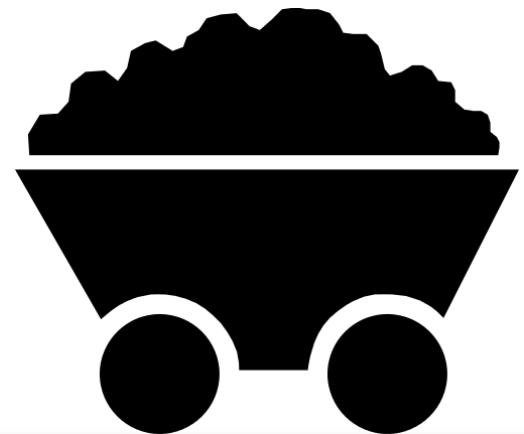
\includegraphics[width=2cm]{images/miner_cart.png}}

